\section{Les concepts et les cadres théoriques}

This chapter opens the «~macro~» half of the module, which studies the
\textbf{politiques conjoncturelles} (\textit{stabilisation policies}): the
policies a State runs to steer the conjoncture. The half has two aims,
«~Comprendre le rôle des politiques conjoncturelles à partir de l'histoire
économique de la France~» and «~Réfléchir aux moyens pour améliorer la
situation actuelle~». Chapter~8 follows those policies through 1970--2026 and
chapter~9 discusses the present French situation; this chapter lays down the
vocabulary and the frameworks both of them use.\\

It moves in three steps. First, what the State is for: the État-gendarme of the
classical economists against the État-providence, and the three fonctions
socio-économiques de l'État that justify intervening at all. Second, the
agrégats of the national accounts --- the produit intérieur brut and its three
calculations, the revenu national brut, the épargne and the besoin de
financement --- and the public finances: budgets,
recettes, prélèvements obligatoires, dépenses, the déficit public and the dette
au sens de Maastricht. Third, the indicators of the economy's déséquilibres
(inflation, croissance, chômage, balance commerciale and balance courante) and
the two ways of steering
it: the stabilisateurs automatiques, which act by themselves, and the
politiques discrétionnaires, budgétaire --- with the Keynesian multiplicateur
derived in full --- and monétaire, with the instruments of the Banque centrale
européenne and the agrégats monétaires it watches.

\subsection{Définition et rôle socio-économique de l'État}

\subsubsection{État gendarme vs.\ État providence}

The two names mark the two ends of a scale: how much the State does beyond
keeping order.

\begin{definition}[État-gendarme (\textit{night-watchman state})]
  Les économistes «~classiques~» (libéraux du XVIII\textsuperscript{e} siècle)
  confient un rôle limité (minimal) à l'État~: l'\textbf{État-gendarme}, qui se
  limite aux \textbf{fonctions régaliennes} (\textit{sovereign functions})~:
  \begin{itemize}
    \item faire la loi et fournir des institutions publiques (marché et droits de
      propriété)~;
    \item faire appliquer la loi (police, justice)~;
    \item battre la monnaie~;
    \item défense et sécurité du territoire.
  \end{itemize}
  Les fonctions régaliennes sont financées par les impôts.
\end{definition}

\begin{definition}[État-providence (\textit{welfare state})]
  L'\textbf{État-providence} désigne~:
  \begin{itemize}
    \item au sens large, l'ensemble des interventions économiques et sociales de
      l'État au-delà du régalien (éducation, assurance maladie, retraites, eau
      potable, infrastructure de transport)~;
    \item dans un sens plus restreint, uniquement l'intervention de l'État dans le
      domaine social, qui vise à assurer un niveau minimal de bien-être à la
      population, en particulier à travers le système de \textbf{protection
      sociale} (\textit{social protection}) (redistribution des richesses et prise
      en charge des risques sociaux).
  \end{itemize}
\end{definition}

The course also gives the English name, Welfare State. The broad sense counts
every intervention beyond the régalien core, schools and transport included; the
narrow sense keeps only the social side --- redistribution and cover against the
risques sociaux --- which is what the protection sociale organises.

\subsubsection{Les 3 fonctions socio-économiques de l'État}

Beyond the régalien core, the course distinguishes three \textbf{fonctions
socio-économiques de l'État} (\textit{socio-economic functions of the state}):

\begin{enumerate}
  \item \textbf{Affectation/\allowbreak allocation des ressources}
    (\textit{allocation of resources}) ($\Rightarrow$ les biens publics et les
    échecs de marché).
    \begin{itemize}
      \item Modifier l'équilibre atteint car il n'est pas optimal en termes
        d'efficacité d'utilisation des ressources des agents (effet externe).
      \item Outils~: offre de services collectifs publics et droit, État-gendarme
        (activités régaliennes), politique de la concurrence, Antitrust, droit de
        la propriété intellectuelle.
    \end{itemize}
  \item \textbf{Répartition} (\textit{distribution}) / redistribution
    ($\Rightarrow$ les solidarités).
    \begin{itemize}
      \item Modifier la répartition des ressources entre les agents pour obtenir
        un équilibre plus conforme à des normes de justice sociale
        (\textbf{prestations sociales} (\textit{social benefits}), subventions).
      \item Outils~: cotisations, taxes $\Rightarrow$ prestations.
    \end{itemize}
  \item \textbf{Relance et stabilisation de la conjoncture} ($\Rightarrow$
    développement économique).
    \begin{itemize}
      \item \textbf{Déséquilibres} (\textit{imbalances}) sur les marchés~: il faut
        restaurer un équilibre stable entre l'offre et la demande.
      \item Outils~: politiques économiques de régulation conjoncturelle
        monétaire ou budgétaire.
    \end{itemize}
\end{enumerate}

The échecs de marché of the first function are the défaillances de marché of
chapter~5, and its effet externe is an externalité: the équilibre de marché is
reached but wastes resources, so the State corrects it. The second function
corrects the répartition rather than the efficiency of the outcome. The third
is the one the rest of this half studies: restoring the balance between supply
and demand with the politiques conjoncturelles, monétaire or budgétaire.

\subsection{Agrégats économiques et finances publiques}

\subsubsection{PIB, balance commerciale, RNB, épargne nationale, investissement national}

\paragraph{Le produit intérieur brut.}

\begin{definition}[Produit intérieur brut (\textit{gross domestic product})]
  Le \textbf{produit intérieur brut} (PIB, ou GDP en anglais) est le principal
  \textbf{agrégat} (\textit{aggregate}) pour mesurer l'activité économique,
  décider de politiques économiques et faire des comparaisons internationales.
\end{definition}

«~Comment on le calcule~?~» The course answers with four conditions:
\begin{itemize}
  \item sur une période donnée~;
  \item pour les \textbf{unités de production résidentes} (\textit{resident
    producer units}) (entreprises), étrangères ou françaises~;
  \item il retient les transactions avec des flux financiers, et aussi la
    production non marchande des administrations publiques, évaluée à son coût~;
  \item il inclut les productions de l'année en cours et la hausse des stocks de
    l'année en cours (pas les reventes d'occasion).
\end{itemize}
The non-market output of the administrations publiques has no sale behind it,
so it enters at what it costs to produce.

\begin{remark}[Formulation du cours]
  «~N'inclut que les transactions avec des flux financiers.~»
\end{remark}

The course then insists that $\text{PIB} \neq \sum$ \textbf{chiffre
d'affaires} (\textit{turnover})~: «~la valeur du PIB est différente de la valeur
de toutes les ventes, sinon on compte deux fois les biens intermédiaires~». What
is added up is the \textbf{valeur ajoutée (VA)} (\textit{value added}) of each
producer, its production minus its \textbf{consommation intermédiaire (CI)}
(\textit{intermediate consumption}), plus the impôts sur les produits net of the
subventions sur les produits:
\[
  \text{PIB} = \sum \text{VA brutes} + \text{impôts sur les produits}
  - \text{subventions sur les produits},
  \qquad \text{VA} = \text{production} - \text{CI}.
\]
The table below shows the adjustment: in 2025,
$2\,664{,}9 + 340{,}5 - 14{,}3 = 2\,991{,}1$~Md€.

\begin{remark}[Formulation du cours]
  «~PIB = Somme des valeurs ajoutées (= production -- consommation
  intermédiaire).~»
\end{remark}

\paragraph{Les 3 calculs du PIB.} The same PIB can be reached three ways, which
give the same total: the \textbf{approche production} (\textit{output
approach}), the \textbf{approche revenus} (\textit{income approach}) and the
\textbf{approche demande} (\textit{expenditure approach}).

\begin{table}[h!]
  \centering
  \small
  \begin{tabularx}{\textwidth}{@{}*{3}{>{\raggedright\arraybackslash}X}@{}}
    \toprule
    Par la production & Par les revenus & Par les dépenses \\
    \midrule
    Valeur ajoutée de toutes les entreprises et les administrations
    & Addition de tous les revenus distribués~: salaires des employés,
      bénéfices des entreprises, revenus de l'État
    & Addition de tout ce qui est acheté~: consommation des ménages,
      investissements des entreprises, dépenses publiques, et exportations moins
      les importations \\
    \bottomrule
  \end{tabularx}
  \caption*{\small Calcul du produit intérieur brut~: les trois approches.
    Each approach counts the same value, seen from production, from the incomes
    it pays or from the spending it meets.}
\end{table}

\begin{table}[h!]
  \centering
  \small
  \begin{tabularx}{\textwidth}{@{}lXrr@{}}
    \toprule
    & & 2024 & 2025 \\
    \midrule
    B1GQ & Produit intérieur brut (approche production) & 2\,935,2 & 2\,991,1 \\
    B1G & \quad Valeur ajoutée brute & 2\,624,9 & 2\,664,9 \\
    D21 & \quad + Impôts sur les produits & 328,8 & 340,5 \\
    D31 & \quad -- Subventions sur les produits & $-18{,}4$ & $-14{,}3$ \\
    \midrule
    B1GQ & Produit intérieur brut (approche demande) & 2\,935,2 & 2\,991,1 \\
    P3 & \quad Dépense de consommation finale & 2\,301,1 & 2\,335,0 \\
    P5 & \quad + Formation brute de capital & 644,8 & 670,4 \\
    P6 & \quad + Exportations de biens et services & 997,0 & 1\,009,4 \\
    P7 & \quad -- Importations de biens et services & 1\,007,7 & 1\,023,8 \\
    \midrule
    B1GQ & Produit intérieur brut (approche revenus) & 2\,935,2 & 2\,991,1 \\
    D1 & \quad Rémunération des salariés & 1\,505,5 & 1\,536,2 \\
    B2A3G & \quad + Excédent brut d'exploitation et revenu mixte brut
      & 1\,036,6 & 1\,046,1 \\
    D2 & \quad + Impôts sur la production et les importations & 458,7 & 473,3 \\
    D3 & \quad -- Subventions & $-65{,}6$ & $-64{,}5$ \\
    \bottomrule
  \end{tabularx}
  \caption*{\small Produit intérieur brut~: les trois approches à prix courants,
    en milliards d'euros (comptes nationaux annuels, base 2020). The subsidy rows
    are printed as negative numbers under a «~--~» label and are subtracted
    once. The three totals agree: le PIB 2025 vaut 2\,991~Md€.}
\end{table}

For economic policy the course keeps the approche demande. Its five rows give
$\text{PIB} = C + I + EX - IM$, where $C$ is the whole consommation finale,
$I$ the investment of ménages, entreprises and État, $EX$ and $IM$ the exports and
imports of goods and services. Splitting the public spending $G$ out of $C$ and
$I$ gives the form the third column of the first table describes, and the one
the multiplicateur below uses:
\[
  \text{PIB} = C + I + G + (EX - IM).
\]
Nous retenons l'approche demande pour les politiques économiques en considérant
le PIB comme la somme de la consommation finale, des investissements des
ménages, entreprises et État et du solde des échanges extérieurs de biens et
services, $EX - IM$. That solde is not the balance courante, which adds to it
the revenus primaires and secondaires exchanged with the reste du monde.

\begin{remark}[Formulation du cours]
  «~\ldots des investissements des ménages, entreprises et État et de la balance
  courante.~»
\end{remark}

\paragraph{Le PIB mesure-t-il la richesse~? \ldots plutôt le RNB.} «~PIB
$\Rightarrow$ la création de valeur est produite DANS le pays par des unités de
production résidant sur le territoire national.~» MAIS~:
\begin{itemize}
  \item une entreprise résidente peut effectuer des travaux à l'extérieur du
    pays~;
  \item la production génère des revenus pour des agents qui ne sont pas
    forcément résidents du pays.
\end{itemize}

\begin{example}[Revenus reçus de l'étranger et versés à l'étranger]
  Exemple~1~: des travailleurs résidents mais de courte durée à l'étranger
  (transfrontaliers, saisonniers, stagiaires).\\
  Exemple~2~: les entreprises françaises payent des dividendes et des intérêts à
  des non résidents et, réciproquement, les résidents français peuvent recevoir
  des intérêts et dividendes de l'étranger.
\end{example}

\begin{definition}[Revenu national brut (\textit{gross national income})]
  $\Rightarrow$ Notion de \textbf{revenu national brut (RNB)}~: ensemble des
  \textbf{revenus primaires} (\textit{primary income}) (salaires et financiers)
  reçus par les unités résidentes en économie ouverte (résidents français et
  étrangers en France et résidents français à l'étranger)~:
  \[
    \text{RNB} = \text{PIB} + \text{revenus reçus du RDM}
    - \text{revenus versés au RDM},
  \]
  où RDM désigne le reste du monde.
\end{definition}

The PIB answers ``where was the value produced?'', the RNB ``who received the
income?''. To measure the richesse of residents, the course prefers the RNB.

\paragraph{Les agrégats.} From the PIB, a cascade of balances leads to the
nation's financing position:
\begin{center}
  \begin{tabular}{@{}rl@{}}
    & PIB + revenus reçus du RDM -- revenus versés au RDM \\
    $=$ & revenu national brut (RNB) \quad (= revenu primaire) \\
    $+$ & transferts courants nets reçus du reste du monde \\
    $=$ & revenu national disponible brut (RNDB) \quad (= revenu secondaire) \\
    $-$ & consommation finale \\
    $=$ & épargne brute \\
    $-$ & investissement \\
    $=$ & besoin ($-$) ou capacité ($+$) de financement de la nation
  \end{tabular}
\end{center}

The \textbf{revenu national disponible brut (RNDB)} (\textit{gross national
disposable income}), or \textbf{revenu secondaire} (\textit{secondary income}),
adds to the RNB the transferts courants nets received from the reste du monde:
the impôts and prestations sociales paid between residents cancel out at the
level of the nation, so only the transfers with non-residents move the RNB to the RNDB. What
the nation does not consume is its \textbf{épargne brute} (\textit{gross
saving}). Once investment is paid for, what is left is either a \textbf{besoin
de financement} (\textit{net borrowing}), if negative, or a \textbf{capacité de
financement} (\textit{net lending}), if positive.

\begin{remark}[Formulation du cours]
  «~= Revenu National Brut (= Revenu primaire) + prestations sociales
  (= transferts de richesse) -- impôts \& taxes = Revenu National Disponible Brut
  (= Revenu secondaire).~»
\end{remark}

This besoin de financement belongs to the whole nation --- ménages, entreprises
and administrations together --- and is not the déficit public, which is the
besoin de financement of the administrations publiques alone (defined below).

\begin{remark}[Formulation du cours]
  «~$\Rightarrow$ Le besoin de financement = Déficit public.~»
\end{remark}

\subsubsection{Finances publiques}

\paragraph{Le budget de l'État vs.\ le budget public.} The State is only one
of the administrations publiques, so two budgets and two balances must be kept
apart.

\begin{definition}[Budget de l'État et budget public]
  Définitions~:
  \begin{itemize}
    \item Le \textbf{budget de l'État} (\textit{state budget}) est composé des
      recettes et des dépenses des administrations centrales.
    \item Le \textbf{budget public} (\textit{general government budget}) est
      composé des recettes et des dépenses de toutes les \textbf{administrations
      publiques (APU)} (\textit{general government})~: État, Sécurité sociale,
      administrations/collectivités territoriales.
    \item \textbf{Solde budgétaire} (\textit{budget balance}) = recettes --
      dépenses de l'État.
    \item \textbf{Solde public} (\textit{general government balance}) = recettes
      -- dépenses publiques totales. Si solde $> 0$, \textbf{excédent budgétaire}
      (\textit{budget surplus}) (public)~; si solde $< 0$, \textbf{déficit
      budgétaire} (\textit{budget deficit}) (public).
  \end{itemize}
\end{definition}

\paragraph{Les finances publiques.} «~L'État (via le ministère du Budget et des
Finances) élabore un budget, c'est-à-dire un document comptable retraçant la
prévision des recettes et dépenses pour une année (à partir d'hypothèses de
croissance, \ldots).~» «~Ce budget est soumis au vote de l'Assemblée nationale
et du Sénat (dans cet ordre), qui peuvent respectivement
amender/accepter/refuser le projet.~» In its decisions the State faces several
constraints:
\begin{itemize}
  \item un endettement limité par les \textbf{critères de Maastricht}
    (\textit{Maastricht criteria}) (1993)~: déficit public $< 3$~\% du PIB et
    \textbf{dette publique} (\textit{public debt}) $< 60$~\% du PIB~; le déficit
    public est notifié à la Commission européenne deux fois par an (fin mars et
    fin septembre)~;
  \item les recettes et les dépenses dépendent de la conjoncture (taxe sur la
    valeur ajoutée (TVA), indemnités chômage\ldots)~;
  \item les recettes sont limitées~: «~trop d'impôt tue l'impôt~»
    (\textbf{courbe de Laffer} (\textit{Laffer curve})).
\end{itemize}
The saying is the courbe de Laffer's: beyond some level, raising the taux d'imposition
brings in less, not more.

\paragraph{Les recettes de l'État en France.} On average, the State's revenue
splits as follows; inside the first block the shares are shares of the
recettes fiscales, and they add up to 100~\%.
\begin{itemize}
  \item \textbf{Recettes fiscales} (\textit{tax revenue}) = impôts (90~\%)~:
    impôt sur le revenu (20~\%), impôt sur les sociétés (IS) (10~\%), TVA
    (50~\%), taxe intérieure de consommation sur les produits énergétiques
    (TICPE), ex-taxe intérieure sur les produits pétroliers (TIPP) (5~\%),
    autres impôts (impôt de solidarité sur la fortune (ISF), droits
    d'enregistrement et de timbre, etc.) (15~\%).
  \item \textbf{Recettes non fiscales} (\textit{non-tax revenue}) (10~\%)~:
    \textbf{recettes du domaine de l'État} (\textit{revenue from state property})
    (Française des jeux, Pari mutuel urbain (PMU), amendes, forêts, revenus locatifs\ldots)~; recettes
    exceptionnelles des privatisations.
\end{itemize}
The ISF no longer exists: it was abolished on 1~January 2018 and replaced by the
impôt sur la fortune immobilière (IFI).

\begin{remark}[Formulation du cours]
  «~Autres impôts (ISF, droits d'enregistrement et de timbres, etc.) (15~\%)~»,
  and the ISF again among the impôts directs.
\end{remark}

\paragraph{Les impôts directs et indirects = prélèvements obligatoires.}

\begin{definition}[Prélèvements obligatoires (\textit{compulsory levies})]
  Les \textbf{prélèvements obligatoires (PO)} sont tous les versements effectués
  par les particuliers et les entreprises aux administrations publiques.
\end{definition}

They are of two kinds.
\begin{itemize}
  \item Les \textbf{impôts directs} (\textit{direct taxes}) sont dus
    nominativement par une personne physique ou morale, qui les supporte
    elle-même~: impôt sur le revenu des personnes physiques (un impôt progressif,
    non proportionnel au revenu), impôt sur les sociétés, ISF (remplacé par
    l'IFI en 2018), cotisations sociales salariales et patronales~; la taxe
    d'habitation et la taxe foncière sont des impôts directs locaux.
  \item Les \textbf{impôts indirects} (\textit{indirect taxes}) sont indépendants
    du revenu~: taxe sur la valeur ajoutée (TVA), taxe intérieure sur les
    produits pétroliers (TIPP), droits de timbre, taxe carbone.
\end{itemize}
What makes a tax direct is who owes and bears it, not its link to income: the
impôt sur les sociétés falls on profits and the ISF on wealth, and the impôt sur
le revenu rises faster than income. The revenus du domaine de l'État are not a
tax at all; they are the recettes non fiscales of the list above.

\begin{remark}[Formulation du cours]
  «~Les impôts directs sont dus nominativement par une personne physique ou
  morale et sont proportionnels au revenu~»~; «~Taxes d'habitation et foncière~»
  and «~revenus du domaine de l'État~» are listed among the impôts indirects.
\end{remark}

The weight of the PO in the economy is the \textbf{taux de PO}
(\textit{tax-to-GDP ratio}):
\[
  \text{taux de PO} = \frac{\text{impôts État} + \text{impôts collectivités
  locales} + \text{cotisations sociales}}{\text{PIB}} \times 100.
\]
In France the taux de PO is around 42--45~\% (43,6~\% in 2025), against
40~\% on average in the Union européenne (UE) and 25~\% in the United States.

\paragraph{Les dépenses publiques en France.}
\begin{itemize}
  \item Les \textbf{dépenses de fonctionnement} (\textit{operating
    expenditure})~: fonctionnement courant des administrations et paye des
    fonctionnaires.
  \item Les \textbf{dépenses en capital} (\textit{capital expenditure})~:
    investissement pour moderniser ou accroître le potentiel productif de l'État.
  \item La dette publique~: la charge de la dette de l'État, c'est-à-dire les
    intérêts et non le remboursement du capital, environ 52~Md€ en 2025.
  \item Les \textbf{dépenses d'intervention} (\textit{intervention expenditure})
    et les subventions~: aide aux entreprises et aux ménages.
  \item Les dépenses militaires.
  \item Les transferts sociaux et européens.
\end{itemize}

\begin{remark}[Formulation du cours]
  «~Remboursement de la dette publique (env.\ 55~Md€ en 2025).~»
\end{remark}

Compared with its neighbours, «~la France dépense plus en \% du PIB que les
autres pays de l'UE sur la santé et la protection sociale~» (2023).

\paragraph{Déficit public et dette au sens de Maastricht.}

\begin{definition}[Déficit public (\textit{public deficit})]
  Le \textbf{déficit public} correspond au besoin de financement des
  administrations publiques. C'est le solde du compte de capital des
  administrations publiques. Il est souvent présenté en termes de points de PIB
  (en \%).
\end{definition}

\begin{definition}[Dette au sens de Maastricht (\textit{Maastricht debt})]
  La \textbf{dette au sens de Maastricht} couvre trois passifs financiers de
  l'ensemble des administrations publiques~:
  \begin{itemize}
    \item les \textbf{numéraires et dépôts} (\textit{currency and deposits})~;
    \item les \textbf{titres de créances} (\textit{debt securities}), négociables
      sur le marché, à court terme comme à long terme~;
    \item les \textbf{crédits} (\textit{loans}), c'est-à-dire les prêts, à court
      ou à long terme.
  \end{itemize}
\end{definition}

The split between the last two is not by échéance: both the titres de créances
and the crédits can be short or long. The titres are traded on the market; the
crédits are prêts.

\begin{remark}[Formulation du cours]
  «~les titres de créances (dette court et moyen termes) (négociables sur le
  marché)~»~; «~les crédits (dette long terme)~».
\end{remark}

«~La durée de vie moyenne de la \textbf{dette négociable} (\textit{marketable
debt}) de l'État en avril 2026 est de 8,5 ans et certains emprunts ont des
échéances à 50 ans.~» That dette négociable is made of the securities the State
issues to cover its besoin de financement. «~Pour financer en partie ce besoin de
financement, l'État se tourne vers les marchés financiers. Plus précisément, il
émet deux types de titres financiers~:
\begin{itemize}
  \item les «~\textbf{bons du Trésor à taux fixe et à intérêt précompté (BTF)}~»
    (\textit{fixed-rate discount Treasury bills}) disposant d'une maturité
    inférieure ou égale à 12 mois, ce qui signifie que ces bons du Trésor sont
    remboursés dans un délai maximum d'un an~;
  \item les «~\textbf{obligations assimilables du Trésor (OAT)}~»
    (\textit{fungible Treasury bonds}) d'une maturité allant de 2 à 50 ans. Il
    s'agit de l'instrument de financement à moyen et long terme de l'État.~»
\end{itemize}
«~La dette et la trésorerie de l'État sont gérées par l'\textbf{Agence France
Trésor (AFT)} (\textit{French Treasury Agency}).~»\\

More generally, les \textbf{titres de créance à court terme}
(\textit{short-term debt securities}) (échéance $< 1$~an) sont les bons du
Trésor, les certificats de dépôt, les billets à ordre et les billets de
trésorerie~; les \textbf{titres de créance à long terme} (\textit{long-term debt
securities}) (échéance $> 1$~an) sont les obligations (OAT). The State's
dette négociable is overwhelmingly long term: at the end of March 2022 it stood
at 2\,210~Md€, of which 151~Md€ of BTF (7~\%) and 2\,058~Md€ of OAT (93~\%), with
a durée de vie moyenne of 8~years and 141~days; at the end of July 2026 it held
220~Md€ at short term and 2\,662~Md€ at medium and long term, 2\,882~Md€ in
all.

\begin{table}[h!]
  \centering
  \small
  \begin{tabularx}{\textwidth}{@{}Xrrrrr@{}}
    \toprule
    Ratio de finances publiques & 2019 & 2022 & 2023 & 2024 & 2025 \\
    \midrule
    Capacité ($+$) ou besoin ($-$) de financement des administrations publiques
      & $-2{,}4$ & $-4{,}7$ & $-5{,}4$ & $-5{,}8$ & $-5{,}1$ \\
    Dette publique (brute)\textsuperscript{1}
      & 97,9 & 111,4 & 109,5 & 112,6 & 115,7 \\
    Dette publique nette\textsuperscript{2}
      & 88,8 & 101,1 & 101,4 & 104,5 & 108,5 \\
    Recettes publiques & 52,8 & 53,7 & 51,4 & 51,2 & 52,2 \\
    Dépenses publiques & 55,2 & 58,4 & 56,8 & 57,0 & 57,3 \\
    Prélèvements obligatoires\textsuperscript{3}
      & 43,9 & 45,0 & 43,2 & 42,7 & 43,6 \\
    \bottomrule
  \end{tabularx}
  \caption*{\small Principaux ratios de finances publiques, en \% du PIB
    (comptes nationaux, base 2020). 1.~Au sens du traité de Maastricht.
    2.~La dette publique nette est égale à la dette publique brute diminuée de
    certains éléments d'actif. 3.~Le taux de prélèvements obligatoires est
    calculé net des crédits d'impôt. Lecture~: en 2025, le besoin de financement
    (ou déficit) des administrations publiques représente 5,1~\% du PIB.}
\end{table}

The \textbf{dette publique brute} (\textit{gross public debt}) of the table is
the dette au sens de Maastricht; the \textbf{dette publique nette}
(\textit{net public debt}) est égale à la dette publique brute diminuée de
certains éléments d'actif. «~Nous voyons que les recettes publiques sont
inférieures aux dépenses publiques $\Rightarrow$ déficit public~»: in 2025 the
recettes reach 52,2~\% of PIB against 57,3~\% for the dépenses, a déficit public
of 5,1~\% du PIB, with a dette brute of 115,7~\% du PIB and a taux de PO of
43,6~\%. The table also shows the déficit rising in 2023 while the dette brute
ratio falls; the question this raises is listed, unanswered, at the end of the
chapter.\\

Finally, who holds that debt: about 52~\% of the French dette publique was held
by non résidents at the end of 2024, the highest share among the G7 countries.

\subsection{Déséquilibres et pilotage de la conjoncture}

To steer the conjoncture one must first measure its déséquilibres. The course
watches four indicators --- the taux d'inflation, the taux de croissance réel, the
taux de chômage, and the balance courante with its balance commerciale --- and
then two ways of acting on
them: the stabilisateurs, which work without any decision, and the politiques
discrétionnaires, which are decisions.

\subsubsection{Les principaux indicateurs}

\paragraph{Inflation, désinflation et déflation.} Prices in the zone euro are
measured by one index. L'\textbf{indice des prix à la consommation de l'Union
monétaire (IPCUM)} (\textit{Monetary Union Index of Consumer Prices}), qui
couvre les pays de la zone euro, est une moyenne pondérée des \textbf{indices
des prix à la consommation harmonisés (IPCH)} (\textit{harmonised index of
consumer prices}) des pays de la zone euro. C'est l'indicateur officiel sur
lequel se base la politique monétaire.

\begin{definition}[Inflation]
  L'\textbf{inflation} est une hausse généralisée et durable de l'indice des prix
  à la consommation (IPCH)~:
  \begin{itemize}
    \item \textbf{inflation rampante} (\textit{creeping inflation}) en dessous de
      10~\%~;
    \item \textbf{inflation galopante} (\textit{galloping inflation}) à partir de
      10~\%~;
    \item \textbf{hyperinflation} au-dessus de 50~\% par mois (seuil de Cagan).
  \end{itemize}
\end{definition}

\begin{definition}[Désinflation (\textit{disinflation})]
  La \textbf{désinflation} est une baisse du taux d'inflation, qui reste
  positif~: les prix montent moins vite.
\end{definition}

\begin{definition}[Déflation]
  La \textbf{déflation} est une baisse généralisée de l'IPCH.
\end{definition}

The three words are easy to confuse. Under désinflation prices still rise, only
more slowly; under déflation they fall. The 10~\% thresholds are annual rates;
the hyperinflation threshold is a monthly one.

\begin{remark}[Formulation du cours]
  «~Hyperinflation au-dessus de 50~\%~»~; «~Désinflation~: ralentissement du
  rythme de croissance de l'inflation~».
\end{remark}

«~L'inflation annuelle cache des variations mensuelles importantes (hausses et
baisses).~» Measured month by month over twelve months, inflation in France
moved between 0~\% and about 2,3~\% from January 2018 to September 2021.

\paragraph{PIB, variations et croissance économique.} PIB = valeur en
milliards d'euros de tous les biens et services produits dans la période
considérée par les résidents. Once more, it is not the sum of the chiffres
d'affaires but $\sum$ VA, plus the impôts sur les produits net of the
subventions sur les produits. Its change from one period to the next is the
\textbf{taux de croissance} (\textit{growth rate}):
\[
  \text{taux de croissance (\%)}
  = \frac{\text{PIB}_t - \text{PIB}_{t-1}}{\text{PIB}_{t-1}} \times 100 .
\]
The denominator is the base period, $t-1$: a change is measured against where it
starts.

\begin{remark}[Formulation du cours]
  «~Taux de croissance (\%) $= \dfrac{\text{PIB}_t - \text{PIB}_{t-1}}
  {\text{PIB}_t} \times 100$~».
\end{remark}

\begin{definition}[Croissance économique (\textit{economic growth})]
  La \textbf{croissance économique} est une variation $> 0$ du PIB entre deux
  périodes.
\end{definition}

\begin{definition}[Ralentissement, récession, crise]
  Le \textbf{ralentissement} (\textit{slowdown}) est une baisse du taux de
  croissance, qui reste positif. La \textbf{récession} (au sens de l'Insee) est un recul du PIB sur au
  moins deux trimestres consécutifs. La \textbf{crise économique}
  (\textit{economic crisis}) correspond à un taux de croissance $< 0$.
\end{definition}

A ralentissement is still croissance; a récession and a crise both mean that
the PIB itself falls.

\begin{remark}[Formulation du cours]
  «~La récession économique = ralentissement du taux de croissance~»~; «~La crise
  économique = variation $< 0$ du taux de croissance entre 2 périodes (sur au
  moins 2 trimestres consécutifs avec hausse du chômage et baisse des
  investissements)~».
\end{remark}

\paragraph{PIB nominal vs.\ PIB réel.} «~Question~: comment savoir lors d'une
variation du PIB s'il y a véritablement croissance ou décroissance~?~»

\begin{example}[Volume et valeur]
  Exemple~1~: la \textbf{production en volume} (\textit{output in volume terms})
  passe de 100 à 120 voitures $\Rightarrow$ hausse de 20~\% en termes réels.\\
  Exemple~2~: la \textbf{production en valeur} (\textit{output in value terms})
  passe de 1\,000~€ à 1\,250~€ en 2023 $\Rightarrow$ hausse de 250~€~? Si les prix
  augmentent de 25~\% et la production en valeur de 25~\%, la production en
  volume ne progresse pas.
\end{example}

«~Si l'on veut mesurer l'évolution réelle de l'activité, il est nécessaire
d'éliminer l'effet de la fluctuation des prix (inflation) $\Rightarrow$ on
regarde le \textbf{taux de croissance réel} (\textit{real growth rate}).~» In the
second example, 25~\% of \textbf{croissance nominale} (\textit{nominal growth})
meets 25~\% of inflation:
\[
  1 + \text{taux de croissance réel}
  = \frac{1 + \text{croissance nominale}}{1 + \text{inflation}}
  = \frac{1 + 0{,}25}{1 + 0{,}25} = 1 + 0{,}00
  \quad\Rightarrow\quad 0~\%.
\]
The \textbf{PIB nominal} (\textit{nominal GDP}) is the PIB en valeur, at the
prices of the year; the \textbf{PIB réel} (\textit{real GDP}) is the PIB en
volume, with the price effect removed. Only the PIB réel says whether more is
produced.\\

The gap between the croissance en valeur (nominale) and the croissance en
volume (réelle) is, approximately, the rise in the price of the PIB, measured by
the déflateur du PIB --- not by the IPCH, which prices consumption only. In
France the gap was wide in the 1970s and early 1980s, when the croissance
nominale ran far above the croissance en volume, and narrow after 1990.

\begin{remark}[Formulation du cours]
  «~Écart entre valeur (nominale) et volume (réel) = taux d'inflation.~»
\end{remark}

Since 2000 the taux de croissance réel of France has been negative only twice,
«~taux réel négatif = crise éco en 2009 et 2020~»: $-2{,}9$~\% in 2009 and
$-7{,}5$~\% in 2020. It was $+0{,}8$~\% in 2025, and the forecast for 2026 is
$+0{,}5$ to $0{,}7$~\%.

\paragraph{Chômage.}

\begin{definition}[Chômage (\textit{unemployment})]
  \textbf{Chômage} selon le \textbf{Bureau international du travail (BIT)}
  (\textit{International Labour Office}), qui permet la comparaison entre les
  pays~: est chômeur une personne de 15 ans ou plus, qui n'a pas travaillé
  pendant une semaine de référence, qui est prête à travailler dans les deux
  semaines à venir et qui est à la recherche active d'un emploi depuis au moins
  quatre semaines ou qui en a trouvé un commençant dans les trois mois à venir.
\end{definition}

France Travail counts something else: the \textbf{demandeurs d'emploi}
(\textit{jobseekers}) registered with it, in five catégories.
\begin{itemize}
  \item Catégorie A~: personne sans emploi qui doit chercher un travail pour
    toucher notamment l'assurance chômage.
  \item Catégories B et C~: personne qui exerce une activité professionnelle à
    temps réduit.
  \item Catégorie D~: personne sans emploi qui n'est actuellement pas disponible
    pour travailler pour des raisons médicales ou de formation.
  \item Catégorie E~: personne qui dispose déjà d'un emploi.
\end{itemize}
Catégories D and E carry no obligation to look for work.

\begin{remark}[Formulation du cours]
  «~une personne de plus de 15 ans~»~; «~Les 5 demandeurs d'emploi selon France
  Travail~».
\end{remark}

\paragraph{Taux de chômage et halo du chômage.} The \textbf{taux de chômage}
(\textit{unemployment rate}) divides the chômeurs au sens du BIT by the
\textbf{population active} (\textit{labour force}), the people in work plus the
chômeurs BIT:
\[
  \text{taux de chômage}
  = \frac{\text{chômeurs au sens du BIT}}
         {\text{population active (= en travail + chômeurs BIT)}} .
\]

\begin{definition}[Halo du chômage (\textit{unemployment halo})]
  \textbf{Halo du chômage} = personnes qui ne disposent pas d'emploi et soit qui
  cherchent activement un emploi, mais ne sont pas disponibles dans les deux
  semaines pour travailler, soit qui veulent travailler, mais n'ont récemment pas
  recherché activement un emploi.
\end{definition}

«~Ainsi, selon le Bureau international du travail, ces personnes ne remplissent
pas les conditions pour être considérées au chômage, mais n'ont pas pour autant
un emploi. Elles appartiennent donc à la population inactive.~» Because the halo
is not counted, the taux de chômage BIT underestimates the real chômage.

\begin{remark}[Formulation du cours]
  «~le halo du chômage aurait tendance à sous-estimer le taux de chômage réel.~»
\end{remark}

«~En moyenne en 2025, 2,5 millions de personnes sont au chômage et 1,9 million
souhaitent travailler, sans pour autant être au chômage au sens du BIT. Elles
forment le «~halo~» autour du chômage.~» The taux de chômage au sens du BIT in
France peaked at about 10,5~\% in the mid-2010s, fell to a low of 7,1~\% in the
first quarter of 2023 and stands at 8,3~\% at the latest point; «~en
comparaison, la France se situe dans la moyenne haute des pays de la zone euro,
où le taux de chômage est de 6,2~\%~», and well above the 5~\% the course takes
as plein emploi.

\paragraph{Quel est le taux de chômage «~minimal~»~?} Not all chômage has the
same cause. Les types de chômage~:
\begin{itemize}
  \item le \textbf{chômage conjoncturel} (\textit{cyclical unemployment}) =
    chômage cyclique~;
  \item le \textbf{chômage structurel} (\textit{structural unemployment}), lié à
    une inadéquation entre les compétences des chômeurs et la demande du marché du
    travail~;
  \item le \textbf{chômage frictionnel} (\textit{frictional unemployment}) ou
    transitionnel, quand une personne veut trouver un nouvel emploi.
\end{itemize}

\begin{definition}[Plein emploi (\textit{full employment})]
  Deux définitions du \textbf{plein emploi}~:
  \begin{itemize}
    \item choix du taux de chômage frictionnel, car c'est un seuil en dessous
      duquel on ne pourra pas descendre. Il correspond aux délais pour qu'un
      travailleur trouve un emploi ou pour qu'un employeur recrute.
      Actuellement, les économistes s'accordent sur un taux de chômage
      frictionnel entre 4,5~\% et 5~\% pour la France. Mais les calculs peuvent
      varier en fonction des hypothèses faites pour le mesurer~!
    \item choix du taux de chômage frictionnel + structurel $\Rightarrow$ le taux
      tourne autour de 7~\%.
  \end{itemize}
\end{definition}

\paragraph{Taux d'activité, taux d'emploi et taux de chômage.} Two more ratios
are taken over the population en âge de travailler (15 to 64):
\begin{itemize}
  \item le \textbf{taux d'activité} (\textit{participation rate}) = population
    active / population en âge de travailler (de 15 ans à 64 ans), environ
    70~\%~;
  \item le \textbf{taux d'emploi} (\textit{employment rate}) = actifs occupés /
    population en âge de travailler~; il mesure le taux d'utilisation de la
    main-d'œuvre.
\end{itemize}
From 1982 to 2022 the taux d'activité, the taux d'emploi and the taux de chômage
move little: «~courbes assez plates et linéaires~».

\paragraph{Composantes de la balance courante.} The external side of the
economy is summed up in the \textbf{balance courante} (\textit{current
account}), the balance des transactions courantes. It has three components:
the commerce de biens, the commerce de services and the revenus. The first two
together form the \textbf{balance commerciale} (\textit{trade balance}) of
goods and services, the $EX - IM$ of the PIB identity. «~Notre balance courante
est plutôt légèrement négative en 2025~»: France runs a deficit on goods, deep
since the mid-2000s, and a surplus on services.\\

Germany is France's main trading partner for exports and imports alike; next
come the imports from China, then the exports and imports of the United States,
Italy, Spain and Belgium, which are fairly close to one another (2025).

\paragraph{Zoom~: impacts des variations du taux de change $e$ sur les
importations et les exportations.} «~Supposons €~= \textbf{monnaie de
référence} (\textit{base currency}) et \$~= \textbf{monnaie de cotation}
(\textit{quote currency}).~» The \textbf{taux de change} (\textit{exchange rate})
$e$ is then quoted as dollars per euro, for instance $e = 1{,}25$~\$/€.
\begin{itemize}
  \item Si la demande d'€ augmente par rapport au \$ $\Rightarrow$ appréciation
    de l'€ par rapport au \$~: on obtient plus de \$ pour 1~€, par exemple
    $e = 1{,}50$~\$/€.
  \item Conséquences~: appréciation de l'€ = baisse des exports et hausse des
    imports~; dépréciation de l'€ = hausse des exports et baisse des imports.
\end{itemize}
An appreciated euro makes French goods dearer abroad and foreign goods cheaper
at home, hence fewer exports and more imports; a depreciation does the
reverse.

\subsubsection{Les stabilisateurs économiques}

\paragraph{Les effets de la conjoncture sur le solde budgétaire.} L'État
contrôle uniquement les taux d'imposition, mais pas le montant total qu'ils
rapportent~: that amount follows the conjoncture.
\begin{itemize}
  \item En période d'expansion, la consommation augmente et donc aussi les
    profits et les revenus. Les recettes fiscales augmentent et les paiements de
    transfert diminuent (allocations chômage) $\Rightarrow$ amélioration
    automatique du solde public.
  \item En période de récession, situation inverse~: dégradation du solde
    public (aides à certains secteurs pour les protéger $\Rightarrow$
    subventions, aides fiscales~; baisse des revenus $\Rightarrow$ baisse des
    recettes fiscales~; hausse des allocations chômage).
\end{itemize}

\begin{figure}[h!]
  \centering
  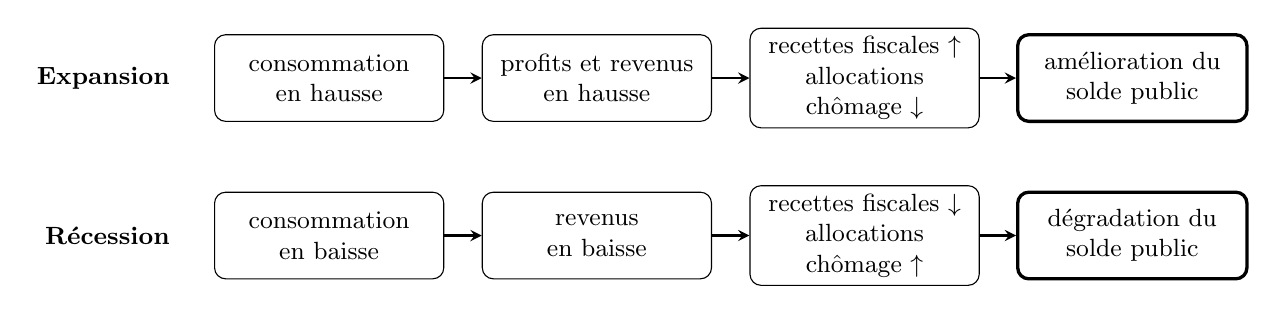
\begin{tikzpicture}[>=stealth, font=\small,
      box/.style={draw, rounded corners, align=center, text width=27mm,
        minimum height=11mm, inner sep=3pt}]
    \node[font=\small\bfseries, anchor=east] at (-0.2,0) {Expansion};
    \node[box] (e1) at (1.7,0) {consommation\\en hausse};
    \node[box] (e2) at (5.1,0) {profits et revenus\\en hausse};
    \node[box] (e3) at (8.5,0) {recettes fiscales $\uparrow$\\allocations
      chômage $\downarrow$};
    \node[box, very thick] (e4) at (11.9,0) {amélioration du\\solde public};
    \draw[->, thick] (e1) -- (e2);
    \draw[->, thick] (e2) -- (e3);
    \draw[->, thick] (e3) -- (e4);
    \node[font=\small\bfseries, anchor=east] at (-0.2,-2) {Récession};
    \node[box] (r1) at (1.7,-2) {consommation\\en baisse};
    \node[box] (r2) at (5.1,-2) {revenus\\en baisse};
    \node[box] (r3) at (8.5,-2) {recettes fiscales $\downarrow$\\allocations
      chômage $\uparrow$};
    \node[box, very thick] (r4) at (11.9,-2) {dégradation du\\solde public};
    \draw[->, thick] (r1) -- (r2);
    \draw[->, thick] (r2) -- (r3);
    \draw[->, thick] (r3) -- (r4);
  \end{tikzpicture}
  \caption*{\small Les stabilisateurs automatiques. The same barème de l'impôt
    and the same allocations chômage turn an expansion into a better solde public and
    a récession into a worse one, with no decision by the State.}
\end{figure}

\begin{definition}[Stabilisateurs automatiques (\textit{automatic stabilisers})]
  Notion de \textbf{stabilisateurs automatiques}, qui jouent par les recettes
  comme par les dépenses publiques~: c'est un mécanisme économique ayant une
  activité régulatrice, passive, et contracyclique immédiate selon la taille des
  transferts (étendue et niveau des allocations chômage, progressivité des
  impôts).
\end{definition}

\begin{remark}[Formulation du cours]
  «~Notion de stabilisateurs économiques automatique des dépenses publiques.~»
\end{remark}

They are passive because nobody decides them: the barème de l'impôt and the
allocations chômage are fixed in advance, and the conjoncture does the rest.
They are contracyclique because the solde public moves against the cycle,
cushioning a downturn with a larger déficit public and cooling an expansion
with a smaller one. Their size depends on how generous the allocations chômage are
and on the progressivité des impôts.

\subsubsection{Les politiques discrétionnaires}

Unlike the stabilisateurs, the \textbf{politiques discrétionnaires}
(\textit{discretionary policies}) are decisions. «~Politiques discrétionnaires de
\textbf{relance} (\textit{stimulus}) ou de \textbf{rigueur} (\textit{restraint})
(ou expansive/restrictive)~»~:
\begin{enumerate}
  \item La \textbf{politique budgétaire} (\textit{fiscal policy})~: en cas de choc
    majeur, les dépenses budgétaires publiques peuvent accélérer le retour à la
    croissance «~normale~».
    \begin{itemize}
      \item Il est possible de moduler les recettes (les impôts) et/ou les
        dépenses (budget public).
      \item \textbf{Politique de la demande} (\textit{demand-side policy})
        $\Rightarrow$ en faveur de la consommation (allègements fiscaux des
        ménages, dépenses publiques de grands travaux) $\Rightarrow$ inspiration
        keynésienne.
      \item \textbf{Politique de l'offre} (\textit{supply-side policy})
        $\Rightarrow$ en faveur des entreprises (allègements fiscaux des
        entreprises, favoriser l'innovation par des subventions, réduire les coûts
        salariaux) $\Rightarrow$ inspiration «~libérale~».
    \end{itemize}
  \item La \textbf{politique monétaire} (\textit{monetary policy})
    $\Rightarrow$ permet de contrôler l'inflation et de soutenir la croissance en
    modifiant la quantité de monnaie en circulation (via la variation des taux
    d'intérêt de court terme).
    \begin{itemize}
      \item Rem.~: la politique de demande keynésienne inclut aussi une politique
        monétaire de relance (baisse des taux) pour favoriser la croissance en
        période d'inflation faible.
    \end{itemize}
\end{enumerate}

\paragraph{Naissance des politiques de relance de l'économie dans les années
1930.} The politiques de relance were born of the crise of 1929.
Origine~: la crise de 1929 aux États-Unis (Jeudi noir du 24 octobre), qui s'est
propagée ensuite en Europe.
\begin{itemize}
  \item \textbf{Krach boursier} (\textit{stock market crash})~: éclatement d'une
    bulle spéculative à Wall Street le jeudi 24 octobre 1929~; la crise se
    propage dans le monde entier.
  \item C'est la \textbf{Grande Dépression} (\textit{Great Depression})~: il
    s'ensuit dix ans de récession économique globale jusqu'au déclenchement de la
    Seconde Guerre mondiale.
\end{itemize}
«~En quelques jours, le cours des actions s'écroule à Wall Street, ruinant des
milliers d'investisseurs et de traders $\Rightarrow$ les banques d'investissement
font faillite, entraînant dans leur chute les entreprises qui ne trouvent plus de
financement.~» The social and economic consequences are disastrous: bankruptcies,
chômage and poverty explode in the United States, where about 25~\% of the
population active was out of work in 1933.

\begin{remark}[Formulation du cours]
  «~30~\% de la population US au chômage.~»
\end{remark}

\paragraph{L'interventionnisme keynésien.} «~Contexte~: crise des années 1930 et
chômage persistant $\Rightarrow$ \textbf{équilibre de sous-emploi}
(\textit{underemployment equilibrium}) $\Rightarrow$ limites de la main invisible
et de la loi des débouchés (Say).~» An équilibre de sous-emploi is an equilibrium
that persists with workers out of work: the market does not bring the economy
back to plein emploi by itself, contrary to the main invisible and to Say's loi
des débouchés.
\begin{itemize}
  \item John Maynard Keynes publie en 1936 son ouvrage \emph{Théorie générale de
    l'emploi, de l'intérêt et de la monnaie} $\Rightarrow$ nouvelles réflexions
    sur le rôle de l'État comme stimulateur de croissance économique.
  \item Keynes propose l'intervention de l'État pour réguler la conjoncture par
    sa politique économique~:
    \begin{itemize}
      \item politique budgétaire expansionniste en période de récession pour
        relancer la demande effective avec accompagnement monétaire (pour limiter
        la hausse des taux d'intérêt) = policy mix (politique budgétaire et
        politique monétaire)~;
      \item politique monétaire restrictive en période de surchauffe pour
        baisser l'inflation.
    \end{itemize}
\end{itemize}

\paragraph{Mécanisme de la politique budgétaire keynésienne de relance par la
demande.} Three notions carry the Keynesian case for a relance budgétaire, and
the last one is its limit.

\begin{definition}[Demande effective (\textit{effective demand})]
  Notion de \textbf{demande effective} chez Keynes = anticipations de
  consommation des ménages, des entreprises, des administrations et des
  exportations. Si les entreprises anticipent plus de débouchés $\Rightarrow$
  hausse de l'investissement $\Rightarrow$ hausse de l'emploi.
\end{definition}

\begin{definition}[Effet multiplicateur (\textit{multiplier effect})]
  Notion d'\textbf{effet multiplicateur} keynésien. \textbf{Multiplicateur des
  dépenses publiques} (\textit{government spending multiplier})~: la hausse des
  dépenses publiques (consommation des administrations) engendre une valeur de
  production supérieure. Explication = \textbf{effet de chaîne} (\textit{chain
  effect})~: lorsque l'État augmente ses dépenses, cela génère des revenus pour
  les agents économiques (entreprises, ménages). Une partie de ces revenus est
  dépensée à son tour, créant ainsi un effet boule de neige.
\end{definition}

The size of the effet multiplicateur follows from a short model. On sait par
l'\textbf{équilibre ressources-emplois} (\textit{supply-use balance}),
ressources (production) = emplois (\textbf{demande globale}
(\textit{aggregate demand})), en économie fermée pour simplifier, que
\[
  Y = C + I + G \qquad (1)
\]
(ou $Y - C = S + T = I + G$, avec $S = Y - T - C$ l'épargne privée). Here the
taxes $T$ sit beside private saving $S$: what households neither consume nor pay
in tax is saved.

\begin{remark}[Formulation du cours]
  «~(ou Y -- C = S = I + G)~».
\end{remark}

Posons
\[
  C = c\,(Y - T) + C_0 \qquad (2)
\]
où $c$ est la \textbf{propension marginale à consommer} (\textit{marginal
propensity to consume}), avec $0 < c < 1$, et $C_0$ la \textbf{consommation
incompressible} (\textit{autonomous consumption}). The bound $0 < c < 1$ is
Keynes's «~\textbf{loi psychologique fondamentale}~» (\textit{fundamental
psychological law})~: quand le revenu augmente, la consommation augmente, mais
moins que le revenu. Only the average share $C/Y$ falls as income rises.

\begin{remark}[Formulation du cours]
  «~loi psycho fondamentale~» = «~quand Y augmente on consomme de moins en
  moins~».
\end{remark}

Posons
\[
  T = tY \qquad (3)
\]
(impôts proportionnels aux revenus), où $t$ est le \textbf{taux marginal
d'imposition} (\textit{marginal tax rate}), avec $0 < t < 1$.

\begin{notation}
  Here $t$ is the taux marginal d'imposition, not the period index of
  $\text{PIB}_t$ in the taux de croissance.
\end{notation}

(2) et (3) dans (1)~:
\[
  Y = c(1 - t)Y + C_0 + I + G
  \iff
  Y = \frac{1}{1 - c(1 - t)} \left[ C_0 + I + G \right].
\]
Impact des dépenses publiques $G$ sur la croissance~:
\[
  \boxed{\ \frac{\partial Y}{\partial G} = \frac{1}{1 - c(1 - t)} > 1\ }
\]
Commentaires~:
\begin{itemize}
  \item plus $t$ est petit et plus $c$ est grand, plus l'effet multiplicateur est
    grand (ceteris paribus)~;
  \item le multiplicateur d'investissement = multiplicateur des dépenses
    publiques~;
  \item le multiplicateur est $> 1$ $\Rightarrow$ une dépense $G$ engendre une
    croissance de $Y$ supérieure à $G$.
\end{itemize}
The multiplicateur exceeds 1 because $0 < c(1-t) < 1$. A larger $c$ means more of
each round of income is spent again; a larger $t$ means more of it leaks into
taxes.

\begin{example}[Et si on baissait les impôts pour relancer la croissance~?]
  Take now the impôt $T$ as forfaitaire: (3) is dropped, and $T$ is a fixed
  amount, exogenous, independent of $Y$ --- no proportional part, $t = 0$. Then
  \[
    Y = c(Y - T) + C_0 + I + G
    \iff
    Y = \frac{1}{1 - c}\left( -cT + C_0 + I + G \right).
  \]
  \begin{itemize}
    \item \textbf{Multiplicateur fiscal} (\textit{tax multiplier})~:
      $\dfrac{\partial Y}{\partial T} = \dfrac{-c}{1 - c}$.
    \item Le \textbf{multiplicateur budgétaire} (\textit{fiscal multiplier})
      devient $\dfrac{\partial Y}{\partial G} = \dfrac{1}{1 - c}$.
    \item On obtient $\left| \dfrac{\partial Y}{\partial T} \right|
      = \dfrac{c}{1 - c} < \dfrac{1}{1 - c}$, car $0 < c < 1$.
  \end{itemize}
  Bilan~: réduire les impôts relance moins la croissance qu'augmenter les
  dépenses publiques dans ce cas $\Rightarrow$ c'est donc moins efficace~! A euro
  of tax cut is first split between consumption and saving, so only $c$ of it
  enters the effet de chaîne; a euro of public spending enters it whole.
\end{example}

\begin{example}[Et si on finançait les dépenses publiques par une hausse des
  impôts équivalente~?]
  On aurait un \textbf{multiplicateur budgétaire équilibré}
  (\textit{balanced-budget multiplier})~: $\partial G = \partial T$ (4). On a
  \[
    Y = \frac{1}{1 - c}\left( C_0 - cT + I + G \right)
    \iff
    \partial Y = \frac{1}{1 - c}(1 - c)\,\partial G \ \text{(d'après (4))}
    \iff
    \frac{\partial Y}{\partial G} = 1 .
  \]
  Bilan~:
  \begin{itemize}
    \item financer par une hausse des impôts n'est plus efficace que baisser les
      impôts seuls que si $c < \tfrac{1}{2}$~: the balanced budget raises $Y$ by
      $\partial G$, a tax cut of the same size by $\tfrac{c}{1 - c}\,\partial G$,
      and $1 > \tfrac{c}{1 - c}$ exactly when $c < \tfrac{1}{2}$~;
    \item la relance budgétaire par l'impôt est moins efficace sur la relance
      qu'un financement par emprunt, MAIS pas de hausse du déficit public~!
  \end{itemize}
\end{example}

\begin{remark}[Formulation du cours]
  «~financer par une hausse des impôts est plus efficace que baisser les impôts
  seuls~».
\end{remark}

The third notion is the limit of a relance financed by emprunt.

\begin{definition}[Effet d'éviction (\textit{crowding-out effect})]
  Notion d'\textbf{effet d'éviction} de l'investissement privé par la dépense
  publique financée par emprunt~:
  \begin{itemize}
    \item financement des dépenses publiques par emprunt (émission de titres sur
      les marchés financiers) $\Rightarrow$ offre de titres en vente $>$ demande
      de titres $\Rightarrow$ baisse des prix des titres pour les rendre
      attractifs (ou hausse du taux d'intérêt)~;
    \item conséquence~: une partie de l'épargne nationale est mobilisée pour la
      dette souveraine au détriment de l'investissement privé $\Rightarrow$ si la
      \textbf{masse monétaire} (\textit{money supply}) reste inchangée (on
      n'annule pas la hausse de $r$), on parle d'effet d'éviction de
      l'investissement privé, dont l'importance dépend du niveau de la hausse de
      $Y$ et de $G$.
  \end{itemize}
\end{definition}

\begin{remark}[Formulation du cours]
  «~effet d'éviction de l'investissement privé par l'investissement public~».
\end{remark}

What crowds out private investment is the borrowing that finances the public
spending, whatever that spending buys, through the rise in $r$. An
accompagnement monétaire that keeps $r$ from rising --- the policy mix of
l'interventionnisme keynésien --- limits it.

\begin{figure}[h!]
  \centering
  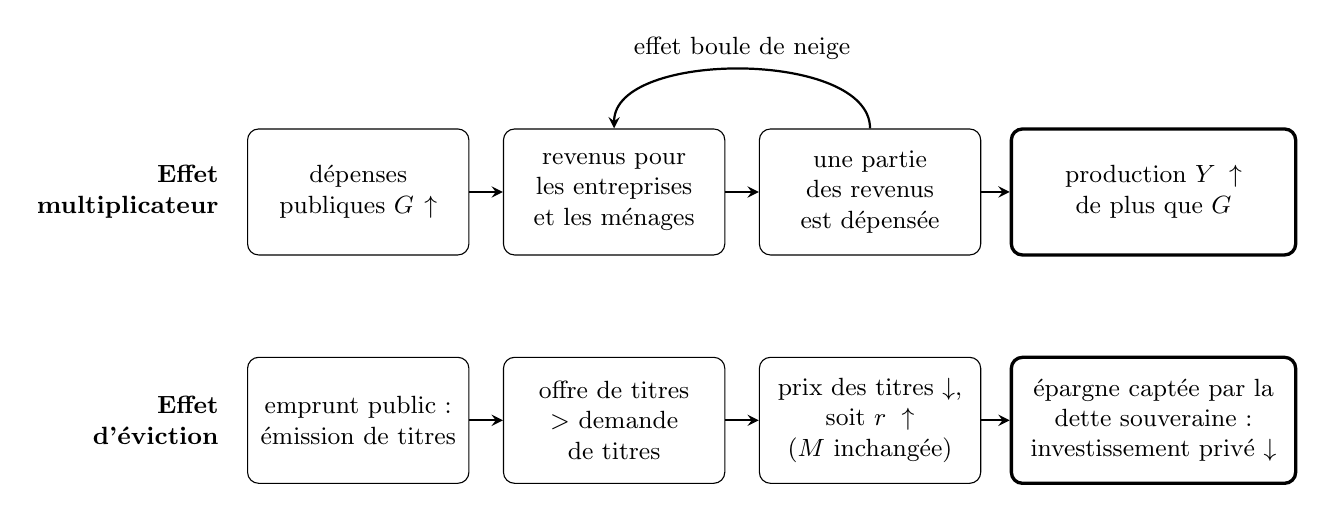
\begin{tikzpicture}[>=stealth, font=\small,
      box/.style={draw, rounded corners, align=center, text width=26mm,
        minimum height=16mm, inner sep=3pt}]
    \node[font=\small\bfseries, align=right, anchor=east] at (-0.2,0)
      {Effet\\multiplicateur};
    \node[box] (m1) at (1.45,0) {dépenses\\publiques $G \uparrow$};
    \node[box] (m2) at (4.7,0) {revenus pour\\les entreprises\\et les ménages};
    \node[box] (m3) at (7.95,0) {une partie\\des revenus\\est dépensée};
    \node[box, very thick, text width=34mm] (m4) at (11.55,0)
      {production $Y \uparrow$\\de plus que $G$};
    \draw[->, thick] (m1) -- (m2);
    \draw[->, thick] (m2) -- (m3);
    \draw[->, thick] (m3.north) .. controls +(0,1.0) and +(0,1.0) ..
      node[above] {effet boule de neige} (m2.north);
    \draw[->, thick] (m3) -- (m4);
    \node[font=\small\bfseries, align=right, anchor=east] at (-0.2,-2.9)
      {Effet\\d'éviction};
    \node[box] (v1) at (1.45,-2.9) {emprunt public~:\\émission de titres};
    \node[box] (v2) at (4.7,-2.9) {offre de titres\\$>$ demande\\de titres};
    \node[box] (v3) at (7.95,-2.9) {prix des titres $\downarrow$,\\soit $r \uparrow$\\($M$ inchangée)};
    \node[box, very thick, text width=34mm] (v4) at (11.55,-2.9)
      {épargne captée par la\\dette souveraine~:\\investissement privé $\downarrow$};
    \draw[->, thick] (v1) -- (v2);
    \draw[->, thick] (v2) -- (v3);
    \draw[->, thick] (v3) -- (v4);
  \end{tikzpicture}
  \caption*{\small Effet multiplicateur et effet d'éviction. Top: each round of
    spending becomes income, part of which is spent again, so the final rise in
    $Y$ exceeds the initial $G$. Bottom: when the spending is financed by
    emprunt and the masse monétaire $M$ stays unchanged, the rise in $r$ diverts
    the épargne nationale from private investment.}
\end{figure}

\paragraph{Politique budgétaire~: comment gérer le déficit~?} A déficit public
can be covered in six ways:
\begin{itemize}
  \item excédents antérieurs~;
  \item patrimoine (privatisations)~;
  \item emprunt --- the BTF and OAT the State issues on the marchés financiers,
    through the AFT~;
  \item hausse de la fiscalité~;
  \item baisse des dépenses publiques~;
  \item exceptionnellement~: par un financement de la Banque centrale européenne
    (assouplissement quantitatif), as in the crise des dettes souveraines of
    chapter~8.
\end{itemize}

\paragraph{La politique monétaire européenne via la BCE.} In the zone euro the
politique monétaire is run by the \textbf{Banque centrale européenne (BCE)}
(\textit{European Central Bank}). Mission~: assurer la \textbf{stabilité des
prix} (\textit{price stability}), un taux IPCH avoisinant 2~\%/an, en
contrôlant la masse monétaire ($M$). Toutes les six semaines, la BCE prend ses
décisions pour maintenir l'inflation à 2~\%~: this 2~\% is the BCE's
\textbf{cible d'inflation} (\textit{inflation target}).\\

What the BCE controls, the masse monétaire, is measured by «~3 agrégats
principaux pour évaluer la monnaie disponible à court terme dans l'économie
($< 2$ ans)~», the \textbf{agrégats monétaires} (\textit{monetary aggregates}):

\begin{definition}[M1, M2, M3]
  Les trois agrégats~:
  \begin{itemize}
    \item \textbf{M1} = \textbf{monnaie au sens strict} (\textit{narrow
      money})~: engagements immédiatement utilisables comme moyens de paiement
      (pièces, billets, \textbf{dépôts à vue} (\textit{demand deposits})). Rem.~:
      dépôts à vue = \textbf{monnaie scripturale} (\textit{bank money}).
    \item \textbf{M2} = M1 + dépôts rémunérés transformables rapidement et sans
      coût en moyens de paiement (Livret~A, compte épargne logement (CEL)).
    \item \textbf{M3} = M2 + pensions + titres d'organismes de placement
      collectif (OPC) monétaires + titres de créance d'une durée $\le 2$ ans émis
      par les institutions financières monétaires (IFM).
  \end{itemize}
\end{definition}

Each agrégat contains the previous one, and what it adds is less and less
liquid, further from a means of payment. M3, the broadest, serves the monetary
analysis of the BCE; inflation itself is measured by the IPCH, not by M3.

\begin{remark}[Formulation du cours]
  The course writes:
  \begin{itemize}
    \item «~M2~: M1 + dépôts rémunérés transformables rapidement et sans coût en
      moyens de paiement (Livret A, CEL, PEL)~»~;
    \item «~M3~: M2 + actifs financiers risqués mais aisément convertibles (SICAV,
      bons du trésor $< 2$ ans)~»~;
    \item «~M3 est le principal agrégat $\Rightarrow$ il est utilisé pour le
      calcul de l'inflation et pour la stratégie de la BCE~».
  \end{itemize}
\end{remark}

\begin{figure}[h!]
  \centering
  \begin{tikzpicture}[>=stealth, font=\small,
      agg/.style={draw, rounded corners, align=left, text width=95mm,
        minimum height=10mm, inner sep=4pt}]
    \node[agg] (m1) at (0,0) {\textbf{M1}~: pièces, billets, dépôts à vue
      (monnaie scripturale)};
    \node[agg] (m2) at (0,-1.45) {\textbf{M2} = M1 + dépôts rémunérés
      transformables rapidement et sans coût (Livret~A, CEL)};
    \node[agg] (m3) at (0,-2.9) {\textbf{M3} = M2 + pensions, titres d'OPC
      monétaires, titres de créance $\le 2$ ans émis par les IFM};
    \draw[->, line width=2.2pt, blue!60] ($(m1.north east)+(0.55,0)$) --
      ($(m3.south east)+(0.55,0)$);
    \node[align=left, anchor=west, text width=27mm]
      at ($(m2.east)+(0.85,0)$) {baisse de la\\liquidité de la\\monnaie};
  \end{tikzpicture}
  \caption*{\small Les agrégats monétaires M1~$\subset$ M2~$\subset$ M3. Reading
    down the list, each agrégat adds to the previous one assets that are less
    liquid, slower or costlier to turn into a means of payment.}
\end{figure}

The BCE acts on $M$ through «~3 canaux~»:
\begin{enumerate}
  \item \textbf{Marché monétaire} (\textit{money market}) ou interbancaire~:
    banques centrales $\Leftrightarrow$ \textbf{banques commerciales}
    (\textit{commercial banks}) $\Rightarrow$ crédits aux
    consommateurs/entreprises~; procurer des espèces aux clients (distributeurs
    automatiques de billets, DAB).
    \begin{itemize}
      \item Modulation sur 3 \textbf{taux directeurs} (\textit{key interest
        rates})~: le \textbf{taux des opérations principales de refinancement}
        (\textit{main refinancing rate}), le \textbf{taux de la facilité de
        dépôt} (\textit{deposit facility rate}) et le \textbf{taux de la
        facilité de prêt marginal} (\textit{marginal lending facility rate}) =
        \textbf{politique monétaire conventionnelle} (\textit{conventional
        monetary policy})~! Une baisse de $r$ augmente l'offre de monnaie.
      \item Les réserves obligatoires (1~\% des engagements des banques d'une
        durée $\le 2$ ans) sont un instrument distinct des taux directeurs.
    \end{itemize}
  \item Banque centrale $\Leftrightarrow$ dette publique (marché secondaire
    seulement)~: the BCE may buy dette publique only on the marché secondaire,
    from other holders, never directly from the Trésor public (article~123 of the
    traité sur le fonctionnement de l'Union européenne, TFUE).
  \item \textbf{Marché des changes} (\textit{foreign exchange market})~: banque
    centrale $\Leftrightarrow$ reste du monde $\Rightarrow$ stabilité du taux de
    change euro/autres devises.
    \begin{itemize}
      \item Rem.~: un pays exportateur net se trouve en situation de
        \textbf{création monétaire} (\textit{money creation}) permanente (hausse
        de la quantité d'euros en circulation via la demande d'euros par le reste
        du monde).
    \end{itemize}
\end{enumerate}

\begin{remark}[Formulation du cours]
  «~taux sur les opérations de refinancement, taux sur les réserve/dépôts auprès
  de la BCE (env.\ 1~\% de leur passif $< 2$ ans), taux facilités de prêt
  marginal~»~; «~Banque centrale $\Leftrightarrow$ Trésor public $\Rightarrow$
  Dette publique (bons du trésor)~».
\end{remark}

Who carries out the création monétaire in the first place? La création
monétaire physique est partagée entre~:
\begin{itemize}
  \item la BCE, qui fixe le volume de billets et de pièces produits par chaque
    pays en fonction des besoins~;
  \item les banques centrales nationales (BCN), qui gèrent le quota de
    \textbf{monnaie fiduciaire} (\textit{currency}) à produire (pièces et
    billets)~;
  \item les banques commerciales ou de second rang (monnaie scripturale/dépôts)~;
  \item le Trésor public (pièces).
\end{itemize}
In the zone euro the coins are issued nationally, by each Trésor public, while
the banknotes are issued by the BCE and the BCN.

\begin{remark}[Formulation du cours]
  «~le Trésor Public (titres de dettes)~».
\end{remark}

«~En France, c'est la Monnaie de Paris qui est chargée de la fabrication des
pièces en euros (usine de Pessac en Gironde). Elle fabrique 800 millions de
pièces courantes par an, dont un tiers de monnaies étrangères.~» «~Il y a 11
imprimeries habilitées pour les billets en Europe (à Clermont-Ferrand en
France).~»

\subsection{Questions de révision}

Eight revision questions on the chapter, each answered from the material above.

\begin{example}[La cible d'inflation de la BCE]
  «~Pourquoi la cible d'inflation de la BCE n'est pas 0~\%~?~» Réponse~: un
  minimum d'inflation est nécessaire pour soutenir l'activité économique et ne
  pas risquer la «~déflation~». Celle-ci est caractérisée par une baisse durable
  des prix qui incite les ménages à reporter leurs décisions de consommation dans
  le temps pour profiter de prix plus bas et qui réduit ainsi la demande adressée
  aux entreprises, au détriment de l'emploi et de l'investissement.\\
  Les taux d'intérêt nominaux pouvant difficilement être significativement
  négatifs, un minimum d'inflation est aussi nécessaire pour abaisser
  suffisamment les taux d'intérêt réels et soutenir ainsi l'activité économique
  lorsque la conjoncture le requiert. Au-delà du minimum nécessaire, l'inflation
  a pour effet de ralentir l'activité économique.\\
  As with growth, a real rate is a nominal rate cleaned of inflation: when the
  nominal rate cannot go much below zero, only some inflation lets the real rate
  go low enough to support activity.
\end{example}

\begin{example}[Le chômage au plein emploi]
  «~Pourquoi le taux de chômage ne vaut pas 0~\% au plein emploi~?~» Because the
  chômage frictionnel is a floor: it reflects «~les délais pour qu'un travailleur
  trouve un emploi ou pour qu'un employeur recrute~», and economists put it
  between 4,5~\% and 5~\% for France. Defined as the taux de chômage frictionnel
  plus structurel, plein emploi sits around 7~\%.
\end{example}

\begin{example}[Le signe de la balance commerciale]
  «~Une balance commerciale doit-elle toujours être positive~? Pourquoi tous les
  pays ne peuvent être tous en excédent commercial~?~» «~Les déficits des pays
  sont les excédents d'autres pays.~» In 2001--2006 the balances courantes
  of China, the major oil exporters, Japan, the other Asian economies (Hong
  Kong, Singapore, Taiwan, Korea, Indonesia, Malaysia) and Russia were in
  surplus, matched by the deficits of the United States --- by far the largest
  --- with Spain, the United Kingdom, Italy and Australia; both sides grew from roughly 400 to 600~billion dollars in 2001 to about
  1\,400~billion in 2006. Since every surplus is someone else's deficit, not
  every country can be in surplus at once, and a positive balance cannot be a
  rule for all.
\end{example}

\begin{example}[Pourquoi une croissance positive]
  «~Pourquoi faut-il une croissance positive (et pas nulle)~?~» Les «~+~» de la
  croissance~:
  \begin{itemize}
    \item lien croissance et prospérité d'un pays~: rôle du progrès technique et
      des innovations sur la qualité de vie~;
    \item lien croissance et stabilité politique et sociale dans un pays~;
    \item innovations et nouvelles ressources~?
    \item plus de ressources publiques~;
    \item remboursement des dettes~;
    \item hausse de l'investissement si innovations ou maximum de productivité~;
    \item hausse de l'emploi~;
    \item hausse de la production~?
    \item prévisions de croissance pour guider les politiques publiques (et le
      budget public).
  \end{itemize}
  And in a period of expansion «~chacun peut espérer voir sa situation
  s'améliorer~», whereas a récession breeds inequalities and social tension.
\end{example}

\begin{example}[Croissance et bien-être]
  «~Est-ce que la croissance augmente le bien-être~?~» Réponse~:
  \begin{itemize}
    \item en période d'expansion, chacun peut recevoir une part des fruits de la
      croissance, c'est-à-dire que chacun peut espérer voir sa situation
      s'améliorer, même si ce n'est pas forcément égalitaire~;
    \item par contre, en période de récession, ceci n'est plus possible
      $\Rightarrow$ inégalités sources de tensions sociales $\Rightarrow$ impact
      sur la cohésion de la société~;
    \item croissance et progrès (technologique, social)~;
    \item croissance et perspectives pour des innovations (start-up,
      investissements)~;
    \item une hausse du PIB d'un territoire ne signifie donc pas mécaniquement une
      amélioration des conditions de vie de ses résidents. La richesse d'un
      territoire ne signifie pas que ses habitants sont eux-mêmes riches
      $\Rightarrow$ cela dépend de la politique redistributive.
  \end{itemize}
  Les «~--~» de la croissance complete the answer~:
  \begin{itemize}
    \item consommation de ressources et production de déchets plus
      importantes~?
    \item la croissance de la richesse produite ne signifie pas un meilleur
      «~welfare state~» (cela dépend de la redistribution~!)~;
    \item satiété des consommateurs~;
    \item la qualité de vie ne dépend pas des biens uniquement monétisables~;
    \item elle ne révèle pas les inégalités sociales~;
    \item risque d'inflation~;
    \item elle n'est pas faite pour évaluer le bien-être.
  \end{itemize}
\end{example}

\begin{example}[Une politique de relance keynésienne]
  «~Expliquer une politique de relance keynésienne.~» In a récession with
  chômage, the State supports the demande effective with a politique de la
  demande: allègements fiscaux des ménages and dépenses publiques de grands
  travaux. Firms that expect more débouchés invest and hire, and the effet
  multiplicateur makes the final rise in production larger than the extra
  spending. If the spending is financed by emprunt, the rise in $r$ threatens an
  effet d'éviction; Keynes therefore pairs the expansionary politique budgétaire
  with an accompagnement monétaire that limits the rise in the taux d'intérêt
  --- the policy mix. In a surchauffe, the politique monétaire turns
  restrictive to bring inflation down.
\end{example}

\begin{example}[L'origine de l'effet multiplicateur]
  «~À quoi est dû l'effet multiplicateur~?~» To the effet de chaîne: the extra
  public spending becomes income for firms and households, a part of which is
  spent in turn and becomes income again. In the model,
  $\dfrac{\partial Y}{\partial G} = \dfrac{1}{1 - c(1 - t)} > 1$, larger when the
  propension marginale à consommer $c$ is high and the taux marginal
  d'imposition $t$ is low.
\end{example}

\begin{example}[Les instruments de la politique monétaire conventionnelle]
  «~Quels sont les instruments de la politique monétaire conventionnelle~?~» The
  three taux directeurs the BCE sets on the marché monétaire --- the taux des
  opérations principales de refinancement, the taux de la facilité de dépôt and
  the taux de la facilité de prêt marginal. A fall in $r$ raises the offre de
  monnaie. The BCE decides every six weeks, to keep inflation near 2~\%; the
  réserves obligatoires are a separate instrument.
\end{example}

\begin{remark}[Questions de révision]
  Questions the course raises and leaves open:
  \begin{itemize}
    \item «~Y a-t-il une contradiction entre la hausse du déficit public en 2023
      et la baisse de la dette publique brute en \% du PIB~?~»
    \item «~Une éco non endettée a-t-elle besoin de croissance~?~»
  \end{itemize}
\end{remark}

\begin{remark}[Concepts clés]
  Les concepts clés à retenir~:
  \begin{itemize}
    \item Fonctions régaliennes vs.\ fonctions socio-économiques de l'État.
    \item Indicateurs clés économiques~: PIB, croissance réelle, inflation,
      chômage, taux de chômage, taux d'emploi, halo du chômage, balance
      commerciale et balance courante.
    \item Indicateurs clés des finances publiques~: les APU, déficit public et
      dette publique, taux de PO.
    \item Les rôles des stabilisateurs automatiques et des politiques
      conjoncturelles.
    \item Les mécanismes de la politique budgétaire (relance keynésienne de la
      demande globale via le multiplicateur, effet d'éviction, politique
      fiscale).
    \item Les mécanismes de la politique monétaire.
  \end{itemize}
\end{remark}
